\chapter{System Description}
\label{sec:system}

In the following the system will be described.
Figure~\ref{fig:system} gives an overview of it.
The transmitters on the left are assumed to be widely spaced, so that they experience no coupling among each other.
The signals are transmittet over a spatial interference channel, therefore a transmitted signal reaches every receiver.
\begin{figure}[h]
\begin{center}
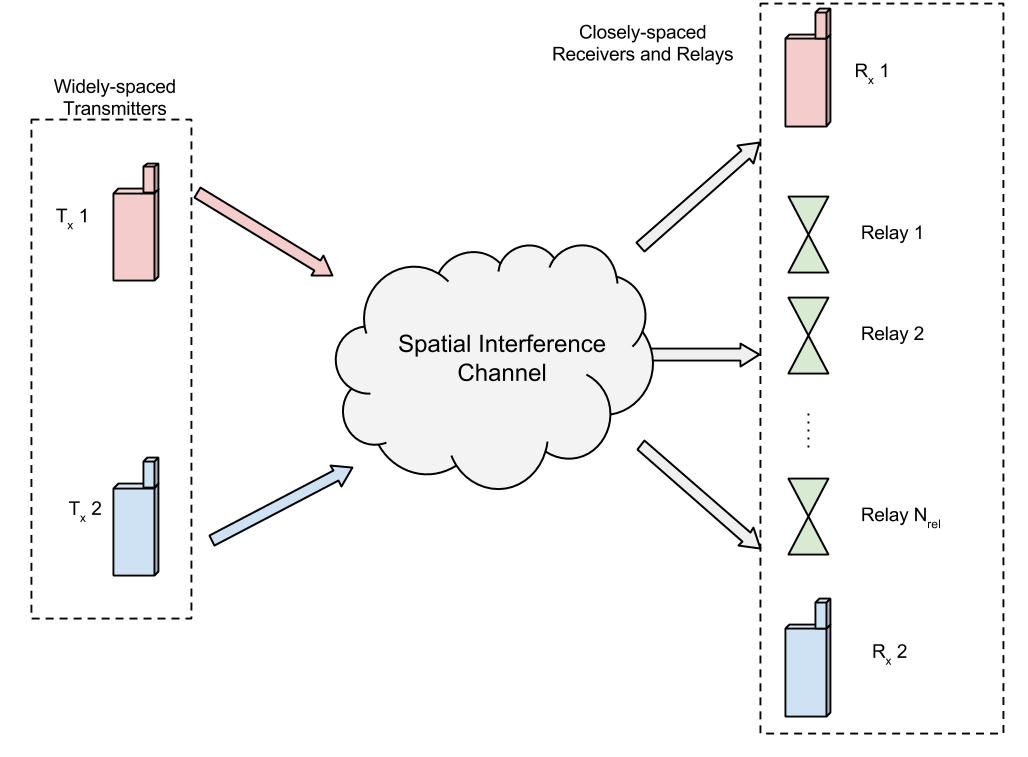
\includegraphics[width=\textwidth]{images/System.png}
\caption{Overview of the system.}
\label{fig:system}
\end{center}
\end{figure}

Besides the receivers themselves, there are passive relays on the right side.
The relays and the receivers are closely spaced, therefore the channels between a transmitter and the receivers and relays are spatially correlated and the elements on the receiver side experience coupling among each other.

\section{Spatial Channel}
\label{sec:spatial}

As mentioned in the previous section the spatial channel is generated by spatial correlation among the receivers and the relays, dependent on the distance.
The correlation matrix is generated by the Besselfuntion according to
\begin{equation}
\label{eq:spatial_corr}
\mat{R}_{i,j} = B(2\cdot d_{i,j}\cdot \pi,0),
\end{equation}
where $B(d,0)$ is the 0-th Besselfunction~\cite[p.191]{Kreyszig} and $d_{i,j}$ the distance between the i-th and j-th receiving element (receive antennas and relays concatenated).
Therefore $\mat{R}$ is symmetric and 1 on its diagonal, as $B(0,0)=1$.

\begin{figure}[h]
\begin{center}
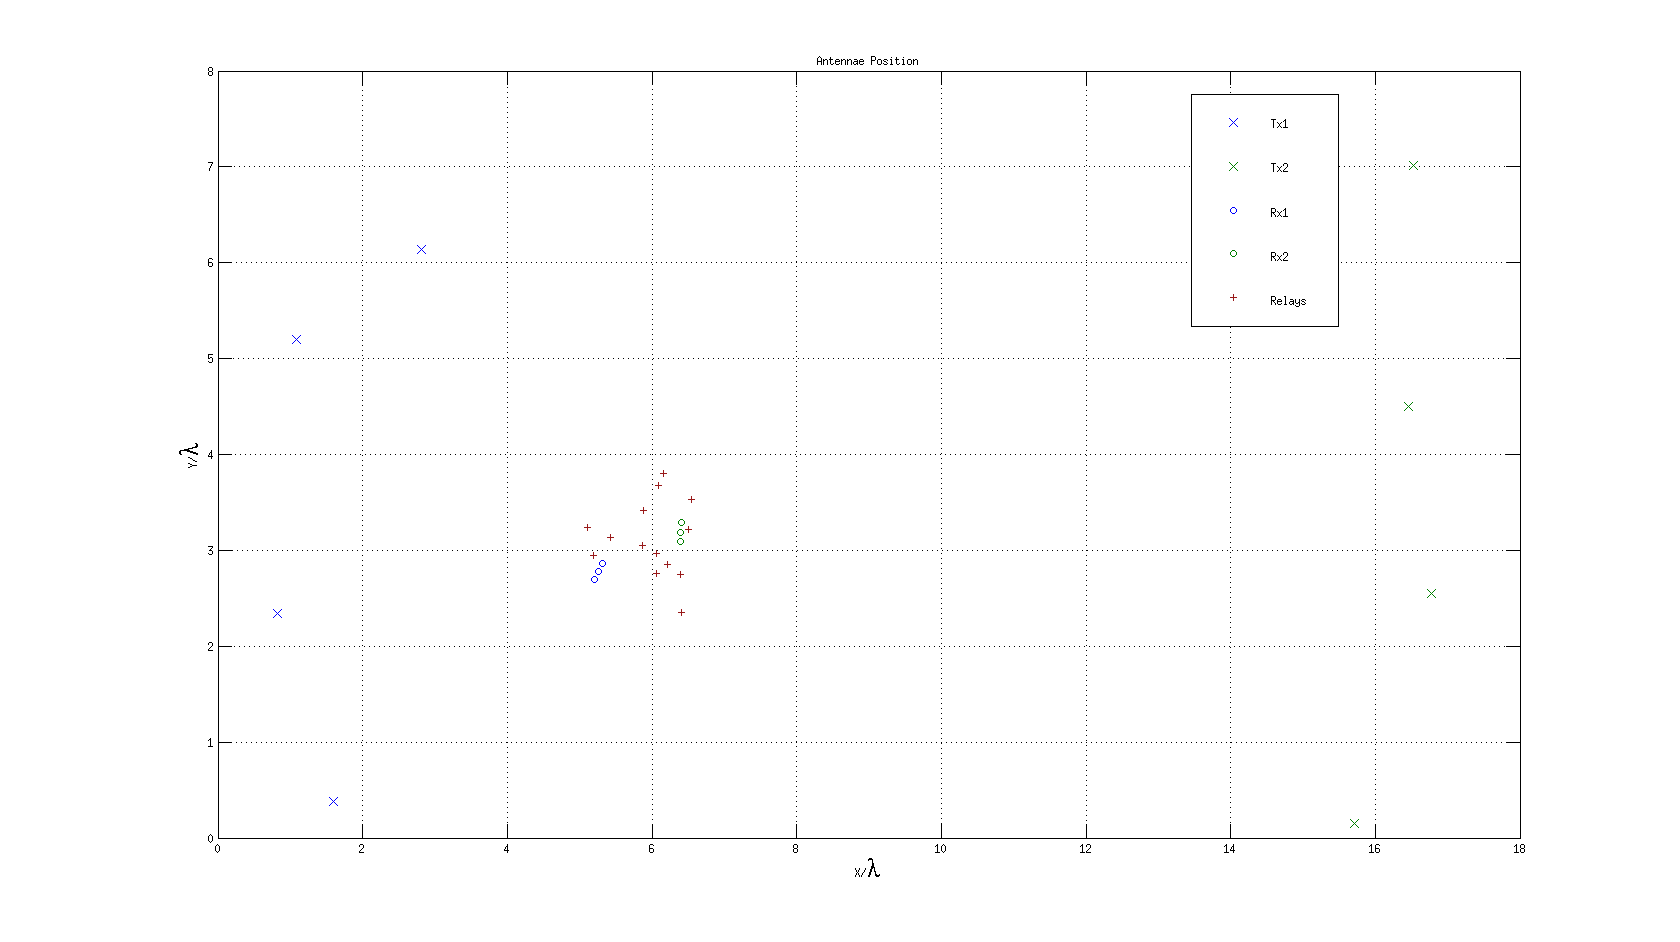
\includegraphics[width=\textwidth]{images/antennae_position.png}
\caption{Example of the receive antenna and the relay placing.}
\label{fig:antenna_placing}
\end{center}
\end{figure}

The spatial channel from $n$-th transmitter to all receivers an relays is then generated by
\begin{equation}
\label{eq:spatial_channel}
\mat{H}_{n}^{\text{sp}} = \mat{R}^{\frac{1}{2}}\cdot\mat{\Delta}_n,
\end{equation} 
where $\mat{\Delta}_n$ is a matrix of size $N_{\text{User}}\cdot \left(N_\text{Rx} + N_\text{Rel}\right) \times N_\text{Tx}$, with complex elements drawn from the standard normal distribution ($\mu = 0$ and $\sigma = 1$).
Therefore $\mat{H}_{n}^{\text{sp}}$ is of size $N_{\text{User}}\cdot \left(N_\text{Rx} + N_\text{Rel}\right) \times N_\text{Tx}$.


\section{Receiver Circuit Description}
\label{sec:network_description}
As mentioned in Section~\ref{sec:SoA}, the idea of describing the receiver circuitry is based on the work of~\cite{Nossek}.
To do so, we represent each receiver block (shown in Figure~\ref{fig:receiver}) by n-ports.
A short overview on 2-ports (simplified n-ports) is given in the following.

\subsection{Multi-Port Networks}
\label{sec:multiport_networks}

In the following a 2-port network will be analyzed.
Later this can be easily extended to a multi-port network.
\begin{figure}[h]
\begin{center}
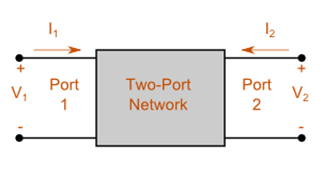
\includegraphics[width=0.75\textwidth]{images/twoport.png}
\caption{A twoport network~\cite{magnus:twoport}.}
\label{fig:twoport}
\end{center}
\end{figure}

Figure~\ref{fig:twoport} shows a 2-port network.
The two-port network can be represented by an impedance matrix $\mat{Z}$.
The elements $Z_{ij}$ of the matrix are defined in the following way:
\begin{align}
\label{eq:multiport_impedance}
Z_{ij} &= \frac{V_i}{I_j},\\\nonumber
&\text{for the currents}\quad I_l = 0,\quad l\neq j.
\end{align}
Therefore the 2-port's input/output relations can be written as
\begin{align}
\label{eq:twoport_io}
\begin{bmatrix}
V_1\\V_2
\end{bmatrix} &= \mat{Z} \cdot
\begin{bmatrix}
I_1\\I_2
\end{bmatrix}
\end{align}

For a multi-port network, elements the voltages and currents can be represented as vectors on length $n$, and the elements $Z_{ij},\quad i,j\in\{1,2\}$ become sub matrices.
Looking from the left into the network with loads $R_L$ attached to the ports on the right, the equivalent input impedance matrix becomes
\begin{equation}
\label{eq:eq_imp_load}
\mat{Z}_{\text{eq}_1} = \mat{Z}_{11} - \mat{Z}_{21}\cdot(\mat{Z}_{22} + R_L\cdot\mat{I})^{-1}\cdot \mat{Z}_{12}.
\end{equation}
With no load attached on port two (open circuited ports, or $R_L\rightarrow\infty$), the equivalent input impedance becomes
\begin{equation}
\label{eq:eq_imp_oc}
\mat{Z}_{\text{eq}_1} = \mat{Z}_{11}.
\end{equation}
Last, having port one short-circuited (i.e.  $R_L\rightarrow 0$) and looking from port two into the network, the equivalent network impedance becomes
\begin{equation}
\label{eq:eq_imp_sc}
\mat{Z}_{\text{eq}_2} = \mat{Z}_{22} - \mat{Z}_{12}\cdot(\mat{Z}_{11})^{-1}\cdot \mat{Z}_{21}.
\end{equation}
For reciprocal networks (\textit{RLC}-Networks, containing only passive elements), following property holds: $\mat{Z}_{12} = \mat{Z}_{21}^T$.

\subsection{Receiver Blocks}
\begin{figure}[h]
\centering
  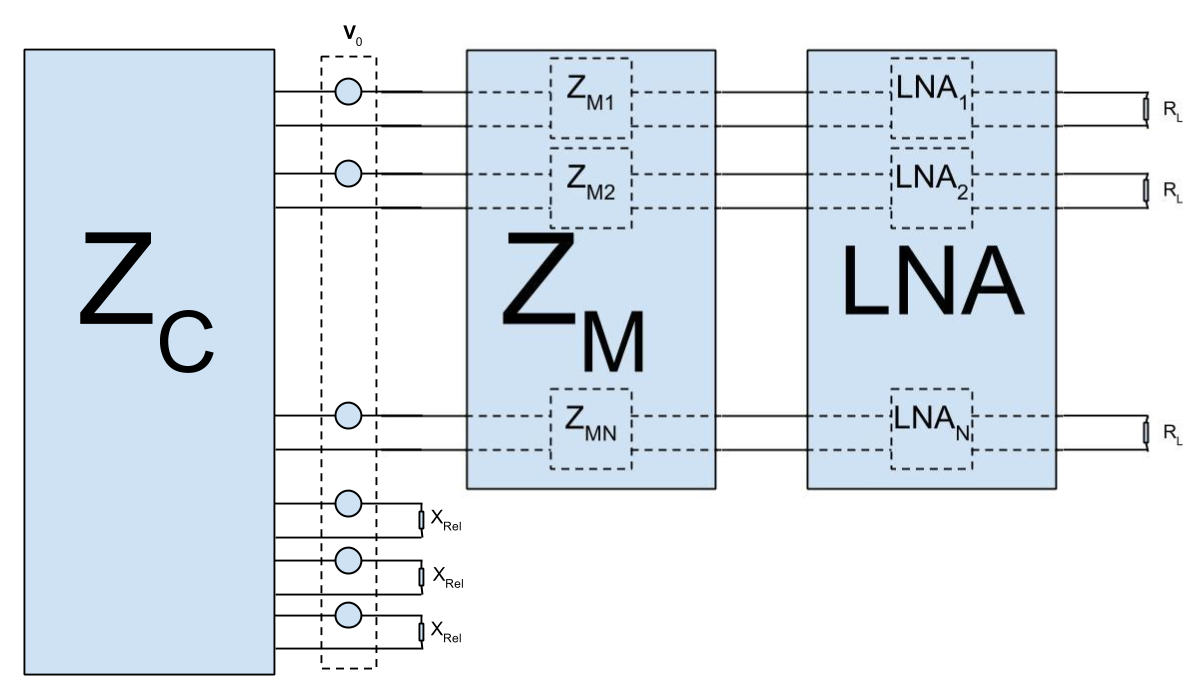
\includegraphics[width=0.9\linewidth]{images/Receiver.png}
\caption{The receiver, with the coupling network $\mat{Z}_\text{C}$, the SP-matching network $\mat{Z}_\text{M}$, the LNA, and loads attached to the LNA.}
\label{fig:receiver}
\end{figure}
The receiver (as shown in Figure~\ref{fig:receiver}) consists of three blocks.
From left to right:
\begin{enumerate}
\item{the coupling network ($\mat{Z}_\text{C}$),}
\item{the matching network ($\mat{Z}_\text{M}$), and}
\item{the low-noise-amplifier ($\mat{LNA}$).}
\end{enumerate}
 
All these blocks can be described in multi-port networks.
In the following each block will be discussed.

\subsubsection{The Coupling Network}
\label{sec:coupling_network}
The coupling network is introduced, as a compact antenna spacing is assumed on the receiver side.
The strength of the coupling between two antennas depends on the spacing between the antennas.
As the effect of coupling from one antenna to another is the same like the reverse, the impedance matrix $\mat{Z}_\text{C}$ becomes symmetric.
The coupling among the antennas is calculated by the "EWA"-Toolbox for MATLAB~\cite{Orfanidis}.
The theory of it can be found in~\cite[Chapter 23]{Orfanidis}.

\subsubsection{The Matching Network}
\label{sec:matching_network}
In order to improve the performance of the receiver, a matching network is placed after each receiving antenna.
For complexity and bandwith reasons, single-port (SP) matching is assumed~\cite{Yahia2013}.
The matching network has the form of 
\begin{equation}
\mat{Z}_\text{M}=
\begin{bmatrix}
\mat{Z}_\text{M11} & \mat{Z}_\text{M12} \\
\mat{Z}_\text{M21} & \mat{Z}_\text{M22}
\end{bmatrix}.
\end{equation}
For a matching network to be lossles it must be pure imaginary and symmetric~\cite{Nossek}.
Because we assume SP matching the submatrices become diagonal, with the choice of a reciprocal network, additionally following property holds: $\mat{Z}_\text{M12} = \mat{Z}_\text{M21}^T \implies \mat{Z}_\text{M12} = \mat{Z}_\text{M21}$.
\begin{figure}[h]
\centering
  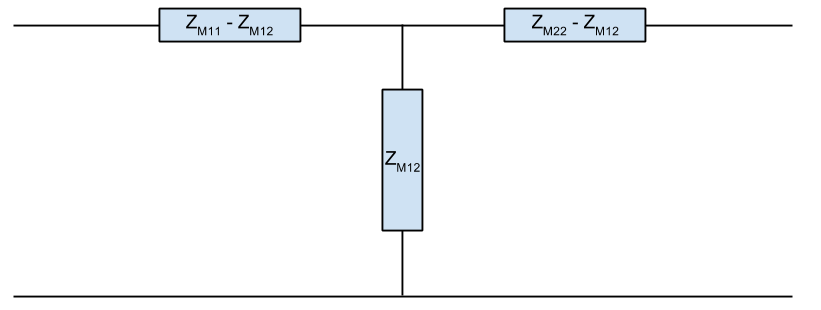
\includegraphics[width=0.7\linewidth]{images/T-Network.png}
\caption{Schematic of a reciprocal T-network.}
\label{fig:t_netw}
\end{figure}

\subsubsection{The Low-Noise-Amplifier}
\label{sec:lna}
In the LNA-block the received signal after the matching network gets amplified.
As in the matchig network the LNA can be represented in the following way
\begin{equation}
\mat{LNA}=
\begin{bmatrix}
\mat{c} & \mat{d} \\
\mat{e} & \mat{g}
\end{bmatrix}.
\end{equation}
As each branch has it's own LNA, the submatrices $\mat{c},\mat{e}\text{ and }\mat{g}$ are again diagonal.
Additionally, matrix $\mat{d}$ is an all-zeros matrix if the unilateral assumtion (\textit{the input of the LNA is not affected by the output of the LNA}) is applied.




\subsection{Port Reduction}
\label{sec:port_reduction}

In the following we describe the open circuit reduction of a system like in Figure~\ref{fig:port_reduction}.
We do the port reduction, because we are interested in the signal only at the loads of the corresponding receiver (here receiver "0").
The signal picked up at relay antennae or not considered receivers contributes to the considered receiver by the coupling between the antennas, as described in Section~\ref{sec:coupling_network}.
The passive relays are modeled by connecting an impedance directly to the coupling network as shown in the lowest 2 branches on the left in Figure~\ref{fig:port_reduction}.
Undesired receivers can be equivalently modeled, however in this case the load corresponds to the equivalent input impedance of the matching network (as in Equation~\eqref{eq:zeqm1}) shown by the third lowest branch on the left.
In the following, $\vec{v}_\text{C}$ denotes the voltages on the ports between the coupling matrix $\mat{Z}_\text{C}$ and the voltage sources $\vec{v}_0$, the same for the currents.
As we are not interested in the input/output-relation of these passive antennas, a port reduction is performed.
For the port reduction, the coupling matrix $\mat{Z}_\text{C}$ can be represented by four submatrices
\begin{equation}
\mat{Z}_\text{C}=
\begin{bmatrix}
\mat{Z}_\text{OO} & \mat{Z}_\text{OL}\\
\mat{Z}_\text{LO} & \mat{Z}_\text{LL}
\end{bmatrix},
\end{equation}
so that we get the system relations

\begin{align}
\label{eq:ocl_matrix}
\begin{bmatrix}
\vec{v}_\text{CO} \\
\vec{v}_\text{CL}
\end{bmatrix}
=
\begin{bmatrix}
\mat{Z}_\text{OO} & \mat{Z}_\text{OL}\\
\mat{Z}_\text{LO} & \mat{Z}_\text{LL}
\end{bmatrix}\cdot
\begin{bmatrix}
\vec{i}_\text{CO} \\
\vec{i}_\text{CL}
\end{bmatrix}.
\end{align}
The index "O" denotes hereby the ports of the required receiver branches, which are open circuited, the index "L" the ports of the non-required receivers and the relays (i.e. the ports with an impedance attached or loaded, respectively).
The indices will change dependent on the user, however without loss of generality, we will derive the port reduction only for user "0" in the following.
We assume, that there are $N_R \cdot N_{Rx}$ antennas, whereby the first $N_{Rx}$ antennas are active (i.e. are the receive antenna of user "0"), and the later ones are passive (i.e. the antennas of the relays and of the other users).
$\mat{Z}_{\text{pass}}$ denotes in the following the $(N_{R}-1)\cdot N_{Rx}$ equivalent input impedances of the non-required receivers and the $N_{Rel}$ impedances representing the relays, placed on the diagonal of a $(N_{R}-1)\cdot N_{Rx}+N_{Rel}$ square matrix.
\begin{figure}[h]
\begin{center}
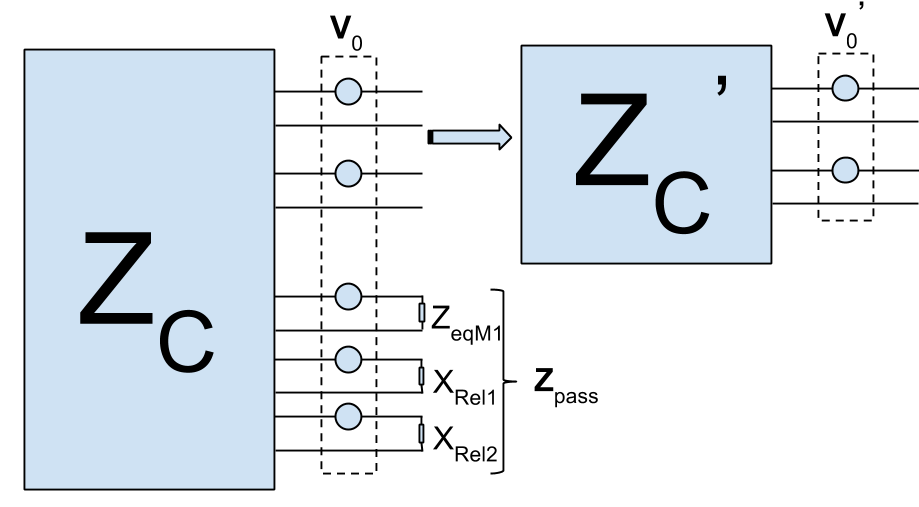
\includegraphics[width=0.75\textwidth]{images/Port_reduction.png}
\caption{Port reduction on a network with one load connected to the last port.}
\label{fig:port_reduction}
\end{center}
\end{figure}

From Equation~\eqref{eq:ocl_matrix} and the property
\begin{align}
\vec{v}_\text{CL} &= \vec{v}_0[N_{Rx}+1:N_R\cdot N_{Rx}]-\mat{Z}_{\text{pass}}\cdot\vec{i}_\text{CL}\quad\text{it follows,}\\
\vec{i}_\text{CL} &= -(\mat{Z}_{\text{pass}} + \mat{Z}_\text{LL})^{-1}\mat{Z}_\text{LO}\cdot\vec{i}_\text{CO} -\\\nonumber
&\qquad (\mat{Z}_{\text{pass}} + \mat{Z}_\text{LL})^{-1}\cdot\vec{v}_{0}[N_i+1:N_R]\\\nonumber\quad\text{and therefore,}&\\
\vec{v}_\text{CO} &= (\mat{Z}_\text{OO}-\mat{Z}_\text{OL}(\mat{Z}_{\text{pass}} + \mat{Z}_\text{LL})^{-1}\mat{Z}_\text{LO})\cdot\vec{i}_\text{CO} -\\\nonumber&\qquad \mat{Z}_\text{OL}(\mat{Z}_{\text{pass}} + \mat{Z}_\text{LL})^{-1}\cdot\vec{v}_0[N_{Rx}+1:N_R\cdot N_{Rx}].
\end{align}
With this port reduction the equivalent coupling matrix and input voltage for user "0" become
\begin{align}
\label{eq:port_reduction}
\mat{Z}_\text{C}^{'}&= \mat{Z}_\text{OO} - \mat{Z}_\text{OL}(\mat{Z}_{\text{pass}} + \mat{Z}_\text{LL})^{-1}\mat{Z}_\text{LO}\quad\text{and}\\
\vec{v}_0^{'} &= \mat{H}_0^{\text{pr}} \cdot\mat{H}_{0}^{\text{sp}}\cdot \vec{v_0}\\\nonumber
&\text{with}\quad\mat{H}_0^{\text{pr}}=
\begin{bmatrix}
\mat{I}_{N_i} & -\mat{Z}_\text{OL}(\mat{Z}_{\text{pass}} + \mat{Z}_\text{LL})^{-1}
\end{bmatrix},
\end{align}
and so we can reduce the system shown in Figure~\ref{fig:receiver}, to a simpler system which only considers the branches of the receiving antenna.











\subsection{Transfer Function of the Receiver}
\label{sec:transf}
The main interest lies in the transfer function of the input voltages $\vec{v}_0$ (without loss of generality we assume user "0" to be the transmitter) to the voltage measured at the loads (in Figure~\ref{fig:receiver}) $\vec{v}_\text{L}$.

In the following the transfer function over each block of the receiver will be derived.
We use the termination: $\vec{v}_i$ is the voltage on the left of the block $i$ (i.e. $v_\text{M}$ is the voltage on the left ports of the matching network).
Additionally, we see the left ports as input ports and the right ports as output ports of each block.
For the derivation of the transfer function we need four equivalent impedance matrices, namely
\begin{enumerate}
\item{$\mat{Z}_{\text{eqM}_1}$, the impedance matrix looking from the left into the matching network,}
\item{$\mat{Z}_{\text{eqM}_2}$, the impedance matrix looking from the right into the matching network,}
\item{$\mat{Z}_{\text{eqLNA}_1}$, the impedance matrix looking from the left into the LNA, and}
\item{$\mat{Z}_{\text{eqLNA}_2}$, the impedance matrix looking from the right into the LNA.}
\end{enumerate}

To calculate $\mat{Z}_{\text{eqM}_1}$ and $\mat{Z}_{\text{eqLNA}_1}$, we use Equation~\eqref{eq:eq_imp_load} and get the following
\begin{align}
\label{eq:zeqm1}
\mat{Z}_{\text{eqM}_1} &= \mat{Z}_\text{M11} - \mat{Z}_\text{M21}\cdot(\mat{Z}_\text{M22} + \mat{Z}_{\text{eqLNA}_1})^{-1}\cdot\mat{Z}_\text{M12},\\
\label{eq:zeqlna1}
\mat{Z}_{\text{eqLNA}_1} &= \mat{c} - \mat{e}\cdot(R_L\mat{I}_{N_R} + \mat{g})^{-1}\cdot\mat{d} = \mat{c}.
\end{align}

As we step through the receiver blocks from left to right, we always have the parallel voltages applied to each receiver block on the left.
Therefore the equivalent input impedances $\mat{Z}_{\text{eqM}_2}$ and $\mat{Z}_{\text{eqLNA}_2}$ can be derived using Equation~\eqref{eq:eq_imp_oc} and lead to the following
\begin{align}
\label{eq:zeqm2}
\mat{Z}_{\text{eqM}_2} &= \mat{Z}_\text{M22} - \mat{Z}_\text{M12}\cdot(\mat{Z}_\text{M11})^{-1}\cdot\mat{Z}_\text{M21},\\
\label{eq:zeqlna2}
\mat{Z}_{\text{eqLNA}_2} &= \mat{g} - \mat{d}\cdot(\mat{c})^{-1}\cdot\mat{e} = \mat{g}.
\end{align}

To get the parallel input voltage on the left of the matching network, we use the principle of a voltage divider as
\begin{equation}
\vec{v_M} = \mat{Z}_{\text{eqM}_1}\cdot(\mat{Z}_{\text{eqM}_1} + \mat{Z}_\text{C})^{-1} \mat{H}_{0}^{\text{sp}}\cdot \vec{v_0}
\end{equation}

To transfer the voltages from the left ports to the right ports of each block we proceed for each block in the following: 
\begin{enumerate}
\item{Calculate the input currents,}
\item{transfer the input currents to the output voltages in series, and}
\item{calculate the output voltages in parallel, by a voltage divider.}
\end{enumerate}
For the matching network, it follows:
\begin{align}
\vec{i_M} &= \mat{Z}_\text{M11}^{-1}\cdot\vec{v_M},\\
\vec{v}_{\text{LNA}_\text{series}} &= \mat{Z}_\text{M12}\cdot\vec{i_M} = \mat{Z}_\text{M12} \mat{Z}_\text{M11}^{-1}\cdot\vec{v_M},\\
\vec{v}_\text{LNA} &= \mat{Z}_{\text{eqLNA}_1}(\mat{Z}_{\text{eqLNA}_1}+\mat{Z}_{\text{eqM}_2})^{-1}\cdot\vec{v}_{\text{LNA}_\text{series}}\\\nonumber
&=\mat{Z}_{\text{eqLNA}_1}(\mat{Z}_{\text{eqLNA}_1}+\mat{Z}_{\text{eqM}_2})^{-1}\mat{Z}_\text{M12} \mat{Z}_\text{M11}^{-1}\cdot\vec{v}_\text{M},
\end{align}
and equivalent for the LNA block
\begin{align}
\vec{v_{L}}&=R_L\mat{I}_{N_R}(R_L\mat{I}_{N_R}+\mat{Z}_{\text{eqLNA}_2})^{-1}\mat{e}\cdot\mat{c}^{-1}\cdot\vec{v}_\text{LNA}.
\end{align}
Therefore we have three transfer functions to characterize our system.
Denoting the transfer function form voltage $\vec{v}_j$ to voltage $\vec{v}_i$ as $\mat{H}_{i,j}$ (i.e. $\vec{v}_i = \mat{H}_{i,j} \cdot\vec{v}_j$), it follows
\begin{align}
\mat{H}_\text{M,0'} &= \mat{Z}_{\text{eqM}_1}\cdot(\mat{Z}_{\text{eqM}_1} + \mat{Z}_\text{C})^{-1}, \\
\mat{H}_\text{LNA,M} &= \mat{Z}_{\text{eqLNA}_1}(\mat{Z}_{\text{eqLNA}_1}+\mat{Z}_{\text{eqM}_2})^{-1}\mat{Z}_\text{M12} \mat{Z}_\text{M11}^{-1},\quad\text{and}\\
\mat{H}_\text{L,LNA} &= R_L\mat{I}_{N_R}(R_L\mat{I}_{N_R}+\mat{Z}_{\text{eqLNA}_2})^{-1}\mat{e}\cdot\mat{c}^{-1}.
\end{align}

And the overall transferfunction
\begin{align}
\label{eq:transf_func}
\mat{H}_\text{L,0'} &= \mat{H}_\text{L,LNA}\cdot\mat{H}_\text{LNA,M}\cdot\mat{H}_\text{M,0'}.
\end{align}



\subsection{Signal Covariance Matrix}
\label{sec:sig_cov}
To calculate the achievable sum rate of the systems (c.f. Section~\ref{sec:rates}), we need to derive the signal covariance matrix, defined as $\mathbb{E}[\vec{v}_\text{L}^s\vec{v}_\text{L}^{s^H}]$.

We assume without loss of generality, that transmitter "0" is the corresponding partner of receiver "0".
The overall transfer functions from $\vec{v}_0$ to $\vec{v}_\text{L}^s$ therefore can be extended from Equation~\eqref{eq:transf_func} to
\begin{align}
\label{eq:transfer_function}
 \vec{v}_\text{L}^s&= \mat{H}_\text{L,LNA}\cdot\mat{H}_\text{LNA,M}\cdot\mat{H}_\text{M,0'}
		\cdot \mat{H}_0^{\text{pr}}\cdot\mat{H}_{0}^{\text{sp}} \cdot\vec{v}_0,\\\nonumber
 &=\mat{H}_\text{L,0}\cdot \mat{H}_{0}^{\text{sp}}\cdot\vec{v}_0,
\end{align}
and hence the signal covariance matrix becomes
\begin{equation}
\label{eq:sig_cov}
\mat{K}_{s,0}=\mathbb{E}[\vec{v}_\text{L}^s\vec{v}_\text{L}^{s^H}] = 
	\mat{H}_\text{L,0}\cdot \mat{H}_{0}^{\text{sp}}
	\cdot\mathbb{E}[\vec{v}_0\vec{v}_0^H]\cdot
	\mat{H}_{0}^{\text{sp}^H} \cdot \mat{H}_\text{L,0}^H,
\end{equation}
where $\mat{H}_\text{L,0}$ is the transfer function including any port reduction at the receiver and $\mat{H}_{0}^{\text{sp}}$ the transferfunction over the spatial channel derived in Equation~\eqref{eq:spatial_channel} for transmitter "0".

\subsection{Interference Covariance Matrix}
\label{sec:int_cov}

To calculate the interference covariance matrix, all the signal sources besides the partner (in this case, all but "0") have to be consider.
This means, that all signal parts arriving at the loads of receiver "0" must be summed up over all the interferer.

The interference covariance matrix hence becomes 
\begin{align}
\label{eq:interf_cov}\nonumber
\mat{K}_{i,0}=\mathbb{E}[\vec{v}_\text{L}^i\vec{v}_\text{L}^{i^H}] &= \sum_{j=1}^{N_\text{User}-1} 
	\mat{H}_\text{L,0} \cdot \mat{H}_{j}^{\text{sp}} \cdot 
	\mathbb{E}[\vec{v}_{j}\vec{v}_{j}^H] \cdot 
	\mat{H}_{j}^{\text{sp}^H} \cdot \mat{H}_\text{L,0}^H,\\
	&= \mat{H}_\text{L,0} \left(\sum_{j=1}^{N_\text{User}-1} 
	\cdot \mat{H}_{j}^{\text{sp}} \cdot 
	\mathbb{E}[\vec{v}_{j}\vec{v}_{j}^H] \cdot 
	\mat{H}_{j}^{\text{sp}^H}\right) \cdot \mat{H}_\text{L,0}^H.
\end{align}


%% Noise part
\section{Noise Description}
\label{sec:noise_description}

As mentioned in~\cite{Yahia2013}, there are four main noise sources in the receiver.
In the following each noise source will be described and its transfer function towards the loads will be derived. 
\begin{figure}[h]
\begin{center}
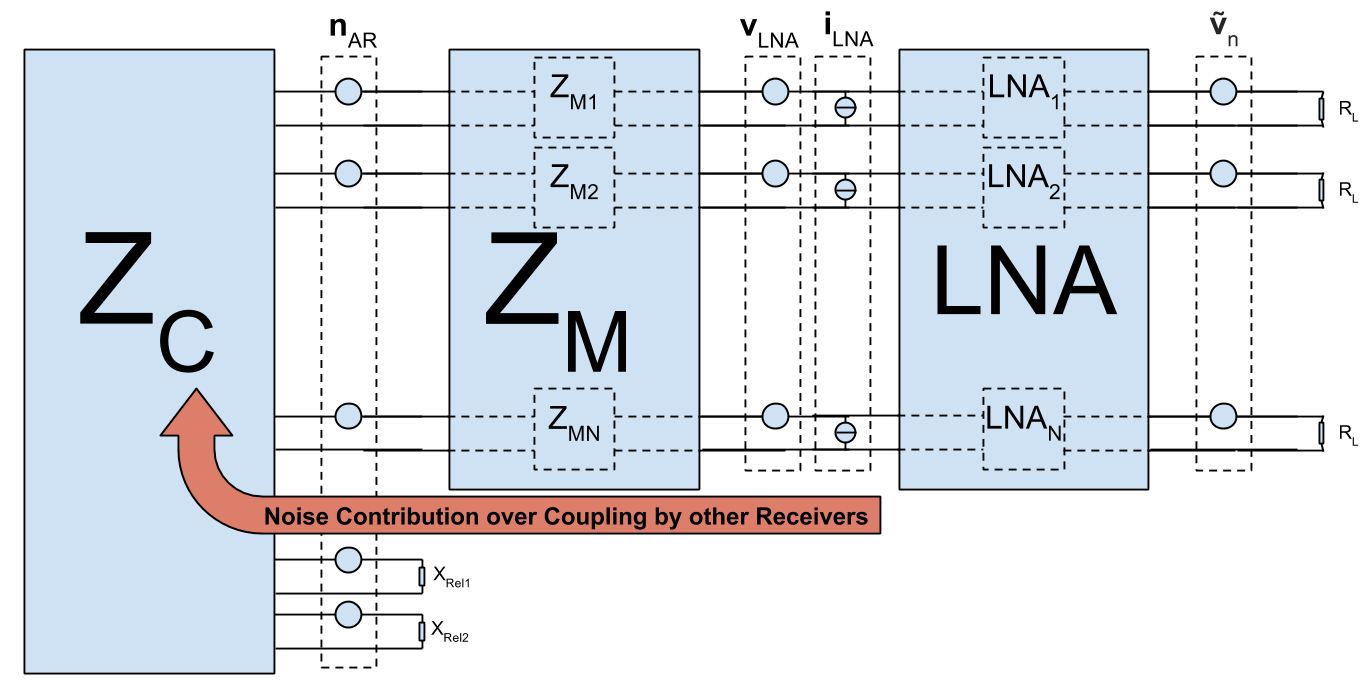
\includegraphics[width=\textwidth]{images/Full_Receiver_noise.png}
\caption{Overview of the system including noise sources.}
\label{fig:receiver_noise}
\end{center}
\end{figure}

Figure~\ref{fig:receiver_noise} gives an overview of the different noise sources.
Important hereby is, that the first three noise sources ($\vec{n}_\text{AR}$, $\vec{v}_\text{LNA}$ and $\vec{i}_\text{LNA}$) also contribute to the other receivers by the coupling.
Only the downstream noise $\vec{\tilde{v}}_n$ is contributing just to its receiver, because of the unilateral assumption of the LNA.

In the following, the transfer functions for the different noise sources will be derived, so that in the end, the total noise contribution at the receiver can be expressed as
\begin{align}\nonumber
\label{eq:noise_contrib}
\vec{u}_\text{L} &= \vec{u}_\text{AR} + \vec{u}_{\text{LNA}_v} + \vec{u}_{\text{LNA}_c} + \vec{u}_{\tilde{n}},\\
&= f(\vec{n}_\text{AR}) + g(\vec{v}_\text{LNA}) + h(\vec{i}_\text{LNA}) + k(\vec{\tilde{v}}_\text{n}),
\end{align}
with $f,g,h,$ and $k$ as the transfer functions for each noise source.

\subsection{Antenna Noise}
\label{sec:antenna_noise}

The antennas introduce two noise sources.
The external noise $\vec{n}_\text{ext}$, collected from the radiation component of the antenna array and the noise generated by the losses in the antennas $\vec{n}_l$.
From~\cite{Twiss1955} it follows, 
\begin{equation}
\label{eq:cov_ant}
\mat{R}_\text{na} = \mathbb{E}[\vec{n}_\text{AR}\vec{n}_\text{AR}^H] = 4 k_B B_W(T_\text{AE}\mathbb{R}\{\mat{Z}_\text{AR}\}+T_\text{AL}\mat{R}_\text{AR}),
\end{equation}
with $k_B$ the Boltzmann constant and $B_W$ the bandwidth.

\subsubsection{Transfer Function of the Antenna Noise}
\label{sec:antenna_noise_transf}
As the antenna noise is picked up by the antennas in the same way as the signal, the transfer function remains the same as the one derived in Equation~\eqref{eq:transfer_function} for the signal, e.g.
\begin{align}
\mat{H}_\text{L,i} &= \mat{H}_\text{L,LNA}\cdot\mat{H}_\text{LNA,M}\cdot\mat{H}_\text{M,O'} \cdot \mat{H}_i^{\text{pr}}.
\end{align}

\subsection{LNA Noise}
\label{sec:lna_noise}

The LNA introduces the third noise source.
From the discussion in~\cite{Nossek}, the noise of the LNA is modeled by a series of voltages and parallel currents at the input of the LNA Block.
The noise sources have the following statistical properties,
\begin{align}
\label{eq:cov_lna}
\mathbb{E}[\vec{i}_\text{LNA}\vec{i}_\text{LNA}^H] &= \beta \cdot \mat{I}_{N_\text{R}N_\text{Rx}},\\\nonumber
\mathbb{E}[\vec{v}_\text{LNA}\vec{v}_\text{LNA}^H] &= \beta \cdot R_n^2\mat{I}_{N_\text{R}N_\text{Rx}},\quad\text{and}\\\nonumber
\mathbb{E}[\vec{v}_\text{LNA}\vec{i}_\text{LNA}^H] &= \rho \beta \cdot R_n\mat{I}_{N_\text{R}N_\text{Rx}},
\end{align}
with $\rho$ and $\beta \cdot$ as correlation coefficients.

\subsubsection{Transfer Function of the LNA Noise}
\label{sec:antenna_noise_transf}
As written above, we have two noise sources, the serial voltage sources and the parallel current sources.
For both of them, we need to consider, that at the loads, we have noise contribution of the LNA of the own receiver branch and LNA noise of the other receiver branches, by the coupling.
Therefore two transfer functions will be derived in the following:
\begin{enumerate}
\item The indirect - a transfer function towards the antenna, and
\item The direct - a transfer function towards the loads.
\end{enumerate}
With the indirect transfer function derived, we can (as in the previous section) concatenate the transfer function of the signal, to get the LNA noise contribution of the other receivers. 

\paragraph{Direct LNA Noise Contribution:}
First we will transfer the current source into a voltage source in series as we then can use the same transfer function for the voltage and the transferred current sources.
To do so, we need the equivalent input impedances looking from the left into the LNA block and from the right into the matching network.
The equivalent input impedance for the LNA network $\mat{Z}_{\text{eqLNA}_1}$ was already derived in~\eqref{eq:zeqlna1}.
To get the equivalent input impedance for the matching network looking from the right into it we use Equation~\eqref{eq:eq_imp_load} and get
\begin{align}
\label{eq:zr}
\mat{\tilde{Z}}_{\text{eqM}_2} &= \mat{Z}_\text{M22} - \mat{Z}_\text{M12}\cdot(\mat{Z}_\text{M11} + \mat{Z}_\text{C'})^{-1}\cdot\mat{Z}_\text{M21}.
\end{align}

Transferring the current source into a series of voltages gives us 
\begin{equation}
\vec{v}_{\text{LNA}_c} = -\mat{\tilde{Z}}_{\text{eqM}_2} \vec{i}_\text{LNA},
\end{equation}

and therefore a transfer function of
\begin{equation}
\label{eq:lnavdir}
\mat{H}_\text{L,LNAv,dir} = R_\text{L}\mat{I}_{N_R}(R_\text{L}\mat{I}_{N_R} + \mat{\tilde{Z}}_{\text{eqLNA}_2})^{-1}\mat{e}\cdot(\mat{c}+\mat{\tilde{Z}}_{\text{eqM}_2})^{-1},
\end{equation}
for the series voltages and
\begin{align}\nonumber
\label{eq:lnacdir}
\mat{H}_\text{L,LNAc,dir} &= -R_\text{L}\mat{I}_{N_R}(R_\text{L}\mat{I}_{N_R} + \mat{\tilde{Z}}_{\text{eqLNA}_2})^{-1}\mat{e}\cdot(\mat{c}+\mat{\tilde{Z}}_{\text{eqM}_2})^{-1}\mat{\tilde{Z}}_{\text{eqM}_2},\\
 &= - \mat{H}_\text{L,LNAv,dir}\cdot \mat{\tilde{Z}}_{\text{eqM}_2},
\end{align}
for the LNA noise currents.
Both transfer functions assume user $i$ to be the receiver.
It is clear to see, that both transfer functions are of size $\mathbb{C}^{N_\text{Rx}\times N_\text{Rx}}$

\paragraph{Indirect LNA Noise Contribution:}
In a second step we transfer the LNA-voltage and -current sources, respectively to parallel voltage sources at the antennas, so that the transfer function derived in Equation~\eqref{eq:transf_func} can be applied.
In the following, all the indices are neglected for simplicity reasons.
For the transfer functions towards the antennas, we consider all the ports of the passive receivers.
Therefore we are looking at matrices of size $\mathbb{C}^{(N_\text{R}-1)N_\text{Rx}\times (N_\text{R}-1)N_\text{Rx}}$.

By multiplying the LNA-current noise source by the equivalent input impedance of the LNA
\begin{align}
\vec{v}_\text{LNAc} = \mat{Z}_{\text{eqLNA1}} \vec{i}_\text{LNA},
\end{align}
it is transferred to a series voltage, just like the LNA-voltage noise.
Now we only need to find the transfer function for the LNA-voltage source $\vec{v}_\text{LNAv}$.
The transfer function over the matching network is given by
\begin{align}
\label{eq:lnanoise_to_input}
\mat{H}_\text{O,LNA} = \mat{Z}_\text{M12}(\mat{Z}_\text{M22}+\mat{Z}_{\text{eqLNA1}})^{-1}.
\end{align}
This leads to the overall indirect LNA noise transfer functions of
\begin{align}
\label{eq:lnaind}\nonumber
\mat{H}_\text{L,LNAv,ind} &= \mat{H}_\text{L,i}\cdot\mat{H}_\text{O,LNA},\quad\text{for the voltage sources, and}\\
\mat{H}_\text{L,LNAc,ind} &= \mat{H}_\text{L,LNAv,ind}\cdot\mat{Z}_{\text{eqLNA1}},\quad\text{for the current sources}.
\end{align}
Looking at the size of the matrices, we see, that the $\mat{H}_\text{O,LNA}$ as well as $\mat{Z}_{\text{eqLNA1}}$ are of size $\mathbb{C}^{(N_\text{R}-1)N_\text{Rx}\times (N_\text{R}-1)N_\text{Rx}}$ and therefore the overall transfer function is of size $\mathbb{C}^{N_\text{Rx}\times (N_\text{R}-1)N_\text{Rx}}$.

\subsection{Downstream Noise}
\label{sec:down_noise}
The last noise source is the downstream noise, generated by all the circuitry after the LNA~\cite{Hughes2012} and modeled by voltage sources $\vec{\tilde{v}}_\text{n}$ in series to the loads.
With the statistical property
\begin{equation}
\label{eq:cov_down}
\mathbb{E}[\vec{\tilde{v}}_\text{n}\vec{\tilde{v}}_\text{n}^H] = \psi\cdot\mat{I}_{N_\text{R}N_\text{Rx}}.
\end{equation}

\subsubsection{Transfer Function of the Downstream Noise}
\label{sec:down_noise_transf}
For the transfer function of the downstream noise we need a simple voltage divider of the loads and the equivalent input impedance $\mat{\tilde{Z}}_{\text{eqLNA}_2}$ looking from the right into the LNA block.
\begin{equation}
\label{eq:down_tf}
\mat{H}_\text{L,n} = R_\text{L}\mat{I}_{N_R}(R_\text{L}\mat{I}_{N_R} + \mat{\tilde{Z}}_{\text{eqLNA}_2})^{-1},
\end{equation}
with 
\begin{align}
\label{eq:zeqlna2_down}
\mat{\tilde{Z}}_{\text{eqLNA}_2} &= \mat{g} - \mat{d}\cdot(\mat{c} + \mat{\tilde{Z}}_{\text{eqM}_2})^{-1}\cdot\mat{e} = \mat{g},
\end{align}
whereby the unilateral assumption ($\vec{d}=\mat{0}$) was applied, and hence $\mat{\tilde{Z}}_{\text{eqLNA}_2}=\mat{Z}_{\text{eqLNA}_2}$ from Equation~\eqref{eq:zeqlna2}.

For the downstream noise we note, that under the unilateral assumption, the transferred noise towards the antennas is zero, because
\begin{align}
\vec{v}_\text{LNAn} = \mat{d}(\mat{g}+R_\text{L}\mat{I}_{N_R})^{-1} \tilde{\vec{v}}_{v}=0,
\end{align}
when $\mat{d}=0$.
Therefore, the downstream noise does only contribute to its own receiver branch, and hence $\mat{H}_\text{L,n}$ is of size $\mathbb{C}^{N_\text{Rx}\times N_\text{Rx}}$.

\subsection{Noise Covariance Matrix}
\label{sec:sig_cov}
In the following we will describe the whole system by its noise transfer functions.
We thereby use the index $i$ for the branches of the active receivers and index $j$ for the branches of the passive receiver, i.e. the branches which contributed only by their coupling.
With the transfer functions derived for each noise source, we can finally express each noise contribution at the loads as stated in Equation~\eqref{eq:noise_contrib} by
\begin{align}
\label{eq:noise_output}
\nonumber
\vec{u}_\text{AR} &= \mat{H}_\text{L,0}\cdot\vec{n}_\text{AR},\\\nonumber 
\vec{u}_{\text{LNA}_v} &= 
	\mat{H}_\text{L,LNAv,ind}\cdot\vec{v}_{\text{LNA},j}+
	\mat{H}_\text{L,LNAv,dir}\cdot\vec{v}_{\text{LNA},i},\\\nonumber
\vec{u}_{\text{LNA}_c} &= 
	\mat{H}_\text{L,LNAc,ind}\cdot\vec{i}_{\text{LNA},j}+
	\mat{H}_\text{L,LNAc,dir}\cdot\vec{i}_{\text{LNA},i},\\\nonumber
\vec{u}_{\tilde{n}} &= \mat{H}_\text{L,n}\cdot\vec{\tilde{v}}_{n},\\
\text{and therefore}\qquad &\vec{u}_\text{L} = \vec{u}_\text{AR} + \vec{u}_{\text{LNA}_v} + \vec{u}_{\text{LNA}_c} + \vec{u}_{\tilde{n}}.
\end{align}

As each vector is of size $\mathbb{C}^{ N_\text{Rx}\times 1}$, the noise covariance matrix, described in the following will be of size $\mathbb{C}^{ N_\text{Rx}\times N_\text{Rx}}$.
Because all the noise sources are uncorrelated, except for the LNA noise sources (c.f. Equation~\eqref{eq:cov_lna}), the noice covariance matrix can be written as:
\begin{align}
\label{eq:exp_noise}\nonumber
\mat{K}_{\text{N,}i} =\mathbb{E}[\vec{u}_\text{L}\vec{u}_\text{L}^H] &=
\mathbb{E}[\vec{u}_\text{AR}\vec{u}_\text{AR}^H]+ 
\mathbb{E}[\vec{u}_{\text{LNA}_v}\vec{u}_{\text{LNA}_v}^H] +
\mathbb{E}[\vec{u}_{\text{LNA}_v}\vec{u}_{\text{LNA}_c}^H] +\\%\nonumber
\quad&\mathbb{E}[\vec{u}_{\text{LNA}_c}\vec{u}_{\text{LNA}_v}^H] +
\mathbb{E}[\vec{u}_{\text{LNA}_c}\vec{u}_{\text{LNA}_c}^H] +
\mathbb{E}[\vec{u}_{\tilde{n}}\vec{u}_{\tilde{n}}^H].
%\mat{K}_{\text{N,}i} =\mathbb{E}[\vec{u}_\text{L}\vec{u}_\text{L}^H] = &\mat{H}_\text{L,i}\mathbb{E}[\vec{n}_\text{AR}\vec{n}_\text{AR}^H]\mat{H}_\text{L,i}^H + 
%\mathbb{E}[\vec{u}_{\text{LNA}_v}\vec{u}_{\text{LNA}_v}^H] +
%\mathbb{E}[\vec{u}_{\text{LNA}_v}\vec{u}_{\text{LNA}_c}^H] +\\%\nonumber
%\quad&\mathbb{E}[\vec{u}_{\text{LNA}_c}\vec{u}_{\text{LNA}_v}^H] +
%\mathbb{E}[\vec{u}_{\text{LNA}_c}\vec{u}_{\text{LNA}_c}^H] +
%\mathbb{E}[\vec{u}_{\tilde{n}}\vec{u}_{\tilde{n}}^H].
\end{align}

For simplicity reasons, we will look in every summand separately in the following.
For the antenna noise it follows therefore
\begin{align}
\mathbb{E}[\vec{u}_\text{AR}\vec{u}_\text{AR}^H] = 
	\mat{H}_\text{L,i}\mathbb{E}[\vec{n}_\text{AR}\vec{n}_\text{AR}^H]\mat{H}_\text{L,i}^H 
	= \mat{H}_\text{L,i} \mat{R}_\text{na} \mat{H}_\text{L,i}^H,
\end{align}
using~\eqref{eq:cov_ant}, with $\mat{R}_\text{na}$ of size $\mathbb{R}^{ N_\text{R}\cdot\left(N_\text{Rx}+N_\text{Rel}\right)\times N_\text{R}\cdot\left(N_\text{Rx}+N_\text{Rel}\right)}$ and hence, by the shape of $\mat{H}_\text{L,i}$, $\mathbb{E}[\vec{u}_\text{AR}\vec{u}_\text{AR}^H]$ becomes a matrix of size $\mathbb{C}^{ N_\text{Rx}\times N_\text{Rx}}$.


For the LNA voltage noise, using~\eqref{eq:cov_lna}, it follows
\begin{align}
\nonumber
\mathbb{E}[\vec{u}_{\text{LNA}_v}\vec{u}_{\text{LNA}_v}^H] &= 
\mathbb{E}[\left(\mat{H}_\text{L,LNAv,ind}\cdot\vec{v}_{\text{LNA},j}+\mat{H}_\text{L,LNAv,dir}\cdot\vec{v}_{\text{LNA},i}\right)\cdot\\
&\qquad\left(\mat{H}_\text{L,LNAv,ind}\cdot\vec{v}_{\text{LNA},j}+\mat{H}_\text{L,LNAv,dir}\cdot\vec{v}_{\text{LNA},i}\right)^H],
\end{align}
by the fact, that $\vec{v}_{\text{LNA},j}$ and $\vec{v}_{\text{LNA},i}$ are independent of each other (c.f. Equation~\eqref{eq:cov_lna}), the cross terms cancel out an hence,
\begin{align}
\nonumber
\mathbb{E}[\vec{u}_{\text{LNA}_v}\vec{u}_{\text{LNA}_v}^H]&=
	\mat{H}_\text{L,LNAv,ind}\cdot
	\mathbb{E}[\vec{v}_{\text{LNA},j}\vec{v}_{\text{LNA},j}^H]\cdot
	\mat{H}_\text{L,LNAv,ind}^H+\\\nonumber
&\qquad \mat{H}_\text{L,LNAv,dir}\cdot
	\mathbb{E}[\vec{v}_{\text{LNA},i}\vec{v}_{\text{LNA},i}^H]\cdot
	\mat{H}_\text{L,LNAv,dir}^H\\
&=\left(\mat{H}_\text{L,LNAv,ind}\cdot\mat{H}_\text{L,LNAv,ind}^H+
	\mat{H}_\text{L,LNAv,dir}\cdot\mat{H}_\text{L,LNAv,dir}^H\right)\cdot \beta \cdot R_n^2.
\end{align}
for the LNA-voltage source and similar for the current source
\begin{align}
\mathbb{E}[\vec{u}_{\text{LNA}_c}\vec{u}_{\text{LNA}_c}^H]&= 
\left(\mat{H}_\text{L,LNAc,ind}\cdot\mat{H}_\text{L,LNAc,ind}^H+
	\mat{H}_\text{L,LNAc,dir}\cdot\mat{H}_\text{L,LNAc,dir}^H\right)\cdot \beta.
\end{align}

The remaining terms for the LNA noise contribution are the cross terms.
For them it follows,
\begin{align}
\nonumber
\mathbb{E}[\vec{u}_{\text{LNA}_c}\vec{u}_{\text{LNA}_v}^H] +&
\mathbb{E}[\vec{u}_{\text{LNA}_c}\vec{u}_{\text{LNA}_c}^H] = 
	\mat{H}_\text{L,LNAv,dir} 
	\cdot\rho\beta \cdot R_n \cdot
	\mat{H}_\text{L,LNAc,dir}^H +\\\nonumber
&\quad	\mat{H}_\text{L,LNAc,dir} 
	\cdot\rho^*\beta \cdot R_n \cdot
	\mat{H}_\text{L,LNAv,dir}^H +\\\nonumber
&\quad	\mat{H}_\text{L,0}\cdot\mat{H}_\text{L,LNAv,ind} 
	\cdot\rho\beta \cdot R_n \cdot
	\mat{H}_\text{L,LNAc,ind}^H\mat{H}_\text{L,0}^H + \\\nonumber
&\quad	\mat{H}_\text{L,0}\cdot\mat{H}_\text{L,LNAc,ind} 
	\cdot\rho^*\beta \cdot R_n \cdot
	\mat{H}_\text{L,LNAv,ind}^H\mat{H}_\text{L,0}^H\\\nonumber
&= \beta \cdot R_n\biggl(
	-\mat{H}_\text{L,LNAv,dir} \left(\rho\mat{\tilde{Z}}_{\text{eqM}_2}^H+
	\mat{\tilde{Z}}_{\text{eqM}_2}\rho^*\right) \mat{H}_\text{L,LNAv,dir}+\\\nonumber
&\quad	\mat{H}_\text{L,LNAv,ind} \left(\rho\mat{Z}_{\text{eqLNA}_1}^H+
	\mat{Z}_{\text{eqLNA}_1}\rho^*\right) \mat{H}_\text{L,LNAv,ind}\biggr)\\\nonumber
&= 2\beta \cdot R_n\biggl(
	-\mat{H}_\text{L,LNAv,dir} \cdot\mathbb{R}\{\rho^*\mat{\tilde{Z}}_{\text{eqM}_2}\}\cdot
	\mat{H}_\text{L,LNAv,dir}+\\
&\quad	\mat{H}_\text{L,LNAv,ind} \cdot\mathbb{R}\{\rho^*\mat{Z}_{\text{eqLNA}_1}\}\cdot
	\mat{H}_\text{L,LNAv,ind}\biggr),
\end{align}
where Equations~\eqref{eq:cov_lna},~\eqref{eq:lnacdir} and~\eqref{eq:lnaind} where used.

Finally, there is only the downstream noise contribution left.
Because of the unilateral assumption, this becomes less complex, i.e.
\begin{align}
\nonumber
\mathbb{E}[\vec{u}_{\tilde{n}}\vec{u}_{\tilde{n}}^H]&=
\psi\left(\mat{H}_\text{L,n}\cdot\mat{H}_\text{L,n}^H\right),
\end{align}
where the statistical property of the downstream noise from Equation~\eqref{eq:cov_down} was used.

With these results we can form the final noise covariance matrix as 
\begin{align}
\label{eq:noise_cov}\nonumber
\mat{K}_{\text{N},i}%&= 
%	\mathbb{E}[\vec{u}_\text{AR}\vec{u}_\text{AR}^H]+
%	\mathbb{E}[\vec{u}_{\text{LNA}_v}\vec{u}_{\text{LNA}_v}^H]+
%	\mathbb{E}[\vec{u}_{\text{LNA}_c}\vec{u}_{\text{LNA}_c}^H]+\\\nonumber
%&\quad	\mathbb{E}[\vec{u}_{\text{LNA}_c}\vec{u}_{\text{LNA}_v}^H] +
%	\mathbb{E}[\vec{u}_{\text{LNA}_c}\vec{u}_{\text{LNA}_c}^H] +
%	\mathbb{E}[\vec{u}_{\tilde{n}}\vec{u}_{\tilde{n}}^H]\\\nonumber
&=\mat{H}_\text{L,i} \mat{R}_\text{na} \mat{H}_\text{L,i}^H+\\\nonumber
&\quad	\beta \cdot R_n^2\cdot \left(\mat{H}_\text{L,LNAv,ind}\cdot\mat{H}_\text{L,LNAv,ind}^H+
	\mat{H}_\text{L,LNAv,dir}\cdot\mat{H}_\text{L,LNAv,dir}^H\right)+\\\nonumber
&\quad	\beta \cdot \left(\mat{H}_\text{L,LNAc,ind}\cdot\mat{H}_\text{L,LNAc,ind}^H+
	\mat{H}_\text{L,LNAc,dir}\cdot\mat{H}_\text{L,LNAc,dir}^H\right)+\\\nonumber
&\quad	2\beta \cdot R_n\biggl(
	-\mat{H}_\text{L,LNAv,dir} \cdot\mathbb{R}\{\rho^*\mat{\tilde{Z}}_{\text{eqM}_2}\}\cdot
	\mat{H}_\text{L,LNAv,dir}+\\\nonumber
&\quad	\mat{H}_\text{L,LNAv,ind} \cdot\mathbb{R}\{\rho^*\mat{Z}_{\text{eqLNA}_1}\}\cdot
	\mat{H}_\text{L,LNAv,ind}\biggr)+\\
&\quad	\psi\left(\mat{H}_\text{L,n}\cdot\mat{H}_\text{L,n}^H\right).
\end{align}
According to the noise vector sizes given in the beginning of this section, the noise covariance matrix is of size $\mathbb{C}^{N_\text{Rx}\times N_\text{Rx}}$.












\section{Rate Calculations}
\label{sec:rates}

\subsection{Achievable Rate}
\label{sec:achiev_rate}
After the derivation of the signal, interference and noise covariance matrix, we can now describe the achievable rate for each connection pair.
The achievable rate for user $j$ is described as
\begin{align}
\label{eq:achiev_rate}
\nonumber
r_j &= \text{log}_2\left(\text{det}\left(\mat{K}_{s,j}\mat{K}_{i,j}^{-1}\mat{K}_{n,j}^{-1}+\mat{I}_{N_R}\right)\right)\\
 &=\text{log}_2\left(\text{det}\left(\mat{K}_{s,j}+\mat{K}_{i,j}+\mat{K}_{n,j}\right)\right) -
	     	\text{log}_2\left(\text{det}\left(\mat{K}_{i,j}+\mat{K}_{n,j}\right)\right).
\end{align}

\begin{align}
\label{eq:achiev_rate}
\nonumber
r_0 &= \text{log}_2\left(\text{det}\left(\mat{K}_{s,0}\mat{K}_{i,0}^{-1}\mat{K}_{n,0}^{-1}+\mat{I}_{N_R}\right)\right)\\
 &=\text{log}_2\left(\text{det}\left(\mat{K}_{s,0}+\mat{K}_{i,0}+\mat{K}_{n,0}\right)\right) -
	     	\text{log}_2\left(\text{det}\left(\mat{K}_{i,0}+\mat{K}_{n,0}\right)\right).
\end{align}

Stacking the achievable rates per user into a vector, leads to 
\begin{equation}
\label{eq:achiev_vec}
\vec{r} =
\begin{bmatrix}
r_1 & r_2 & \cdots & r_N
\end{bmatrix}^T.
\end{equation}

And by this vector we can describe the achievable sum rate as
\begin{equation}
\label{eq:achiev_sum_rate}
r_\text{Sum} = ||\vec{r}||_1,
\end{equation}
with $||\cdot||_1$ the 1-norm, i.e. the sum of the elements of $\vec{r}$.

\subsection{Interference Limited Rate}
\label{sec:sir_rate}
Another measure required in this thesis is the interference limited rate.
It is calculated by only considering the signal and interference.
Therefore neglecting the noise in Equation~\ref{eq:achiev_rate} leads to
\begin{align}
\label{eq:sir_rate}
r_j &=\text{log}_2\left(\text{det}\left(\mat{K}_{s,j}+\mat{K}_{i,j}\right)\right) -
	     	\text{log}_2\left(\text{det}\left(\mat{K}_{i,j}\right)\right).
\end{align}

This is helpful, to see how good the interference was removed by the optimization, which will be introduced in Chapter~\ref{sec:solver}.



\subsection{TDMA Rate}
\label{sec:tdma_rate}
In the later sections the results achieved in this thesis will be compared to existing protocols eliminating interference, such as TDMA.
Therefore in the following the the achievable rates for the TDMA protocol will be shown.

As the time in TDMA is split up in slots in which each user is allowed to transmit without any interference, the achievable rate from Equation~\eqref{eq:achiev_rate} reduces to the interference free achievable rate of 
\begin{align}
\label{eq:tdma_achiev_rate}
r_j  &=\frac{1}{N_\text{User}}\cdot\left(
		\text{log}_2\left(\text{det}\left(\mat{K}_{s,j}+\mat{K}_{n,j}\right)\right) -
	     	\text{log}_2\left(\text{det}\left(\mat{K}_{n,j}\right)\right)\right).
\end{align}
It is obvious, that with no interference, this rate would be higher than the achievable rate with interference, if the factor of $\frac{1}{N_\text{User}}$ was not considered.
However each user is not allowed anymore, to use the full transmission period, but only a time slot of length $\frac{1}{N_\text{User}}\cdot T_0$, with $T_0$ the length of the full transmission period.
Therefore the achievable sum rate can be written as
\begin{align}
\label{eq:tdma_achiev_sum_rate}
\nonumber
r_\text{Sum} &= ||\vec{r}||_1,\\
&= \frac{1}{N_\text{User}}\cdot \sum_{j=0}^{N_\text{User}-1} r_j.
\end{align}
The term $\frac{1}{N_\text{User}}$ is hereby called "pre-log" factor and the reason why TDMA is not a good approach for a large number of users, as $N_\text{User}$ increases linearly, however the advantage of an interference free link will only increase the rate logarithmically over a low interference connection.

There are different approaches of using TDMA, such as allowing a small number of users at the same time to transmit during one time slot.
This will lead to some interference but therefore also a smaller pre-log factor.
Such an approach is used in the later chapters.





